\documentclass{beamer}

\usepackage[portuguese]{babel}
\usepackage{graphicx}
\usepackage{caption}
\usepackage{ragged2e}

\usepackage{tikz}
\usetikzlibrary{positioning}

\usefonttheme{serif}
\beamertemplatenavigationsymbolsempty

\title{Autoencoders}
\author{Eduardo de Medeiros da Silveira}
\institute{Universidade Federal de Santa Maria}
\date{}

\begin{document}

\frame{\titlepage}

\begin{frame}{Representação Eficiente de Dados}

	\justifying

	Em 1970, William Chase and Herbert Simon fizeram um experimento com jogadores profissionais de xadrez, para estudar a relação entre memória, percepção e reconhecimento de padrões.

	\begin{itemize}
		\item<2-> Capazes de memorizar o tabuleiro em poucos segundos.
		\item<3-> Somente quando as peças estavam em posições naturais.
		\item<4-> O reconhecimento de padrões ajuda na memorização.
	\end{itemize}

\end{frame}

\begin{frame}{Representação Eficiente de Dados}

	\begin{figure}

		\centering

		\begin{tikzpicture}

			\node[inner sep=0, outer sep=0] (chess-left) at (-3.5,0) {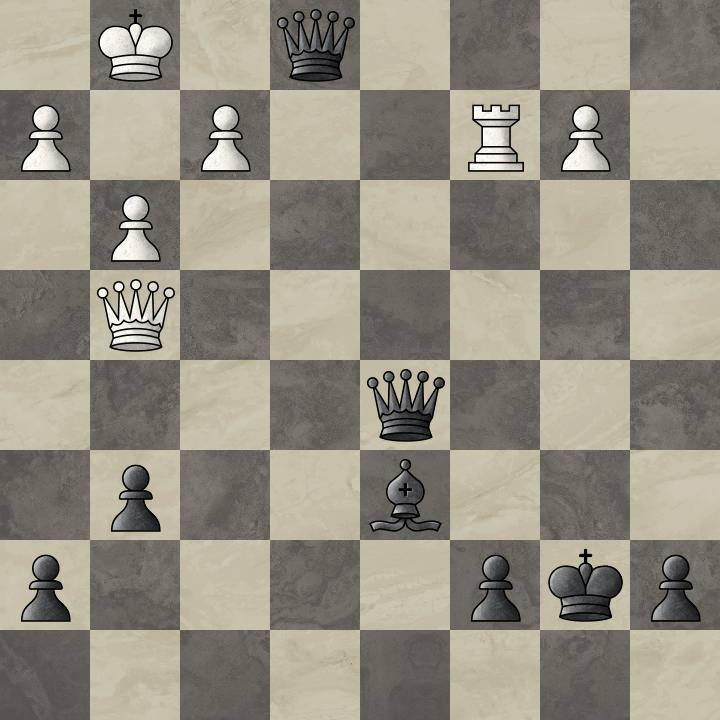
\includegraphics[width=.25\textwidth]{img/chess.jpeg}};
			\node[inner sep=0, outer sep=0, align=center] at (-3.5, 1.6) {Percepção};

			\node[inner sep=0] (abstract) at (0,0) {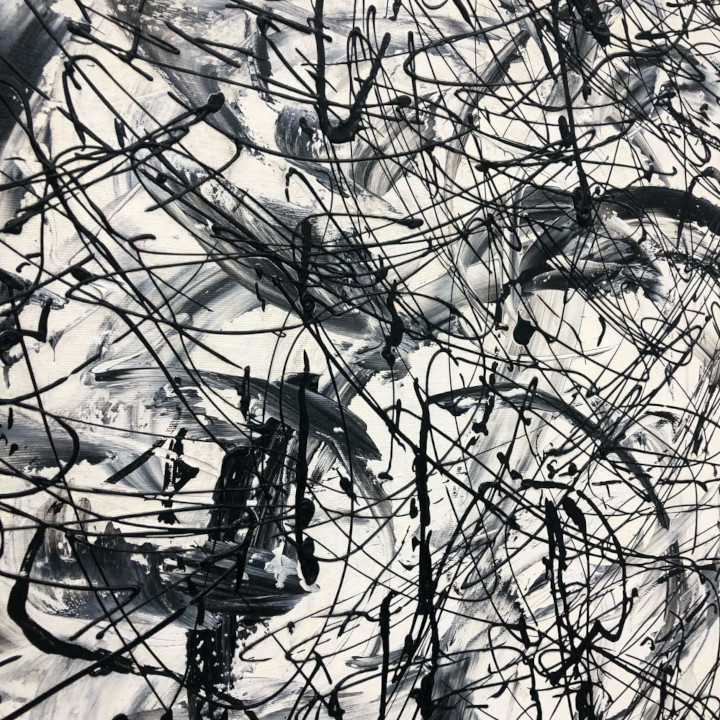
\includegraphics[width=.25\textwidth]{img/abstract.jpg}};
			\node[inner sep=0, outer sep=0, align=center] at (0, 1.6) {Memorização};

			\node[inner sep=0] (chess-right) at (3.5,0) {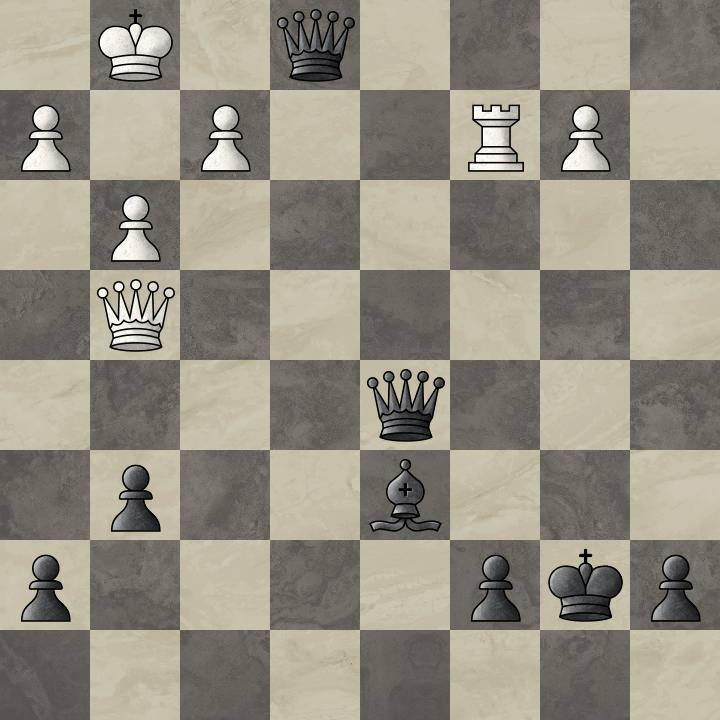
\includegraphics[width=.25\textwidth]{img/chess.jpeg}};
			\node[inner sep=0, outer sep=0, align=center] at (3.5, 1.6) {Recordação};

			\draw[->, thick] (chess-left.east) -- (abstract.west) node[midway, above] {};
			\draw[->, thick] (abstract.east) -- (chess-right.west) node[midway, above] {};

		\end{tikzpicture}

		\caption{Etapas do experimento da memória no xadrez.}

	\end{figure}

\end{frame}

\begin{frame}{Autoencoder}

	\justifying

	Um \emph{autoencoder} é uma rede neural que \textbf{tenta} aprender a função identidade.

	\begin{figure}

		\centering

		\begin{tikzpicture}[
				roundnode/.style={circle, draw=black, minimum size=10mm}
			]

			\node[roundnode] (hidden) {$\boldsymbol{h}$};
			\node[roundnode] (input) [below left=of hidden] {$\boldsymbol{x}$};
			\node[roundnode] (output) [below right= of hidden] {$\boldsymbol{x'}$};

			\draw[->] (input.north east) -- node[pos=0.35, above] {$f$} (hidden.south west);
			\draw[->] (hidden.south east) -- node[pos=0.65, above] {$g$} (output.north west);

		\end{tikzpicture}

		\caption{
			\justifying
			Esquema geral de um \emph{autoencoder}, que mapeia uma entrada $\boldsymbol{x}$ para uma saída $\boldsymbol{x'}$, através de uma representação interna $\boldsymbol{h}$.
			O \emph{autoencoder} é composto por um codificador $f$ e um decodificador $g$.
		}

	\end{figure}

\end{frame}

\begin{frame}{Autoencoder}

	Algumas características:

	\begin{itemize}
		\item<2-> Aprendizado (auto-)supervisionado.
		\item<3-> Perceptron de múltiplas camadas (geralmente).
		\item<4-> Mesmo número de neurônios na entrada e na saída.
		\item<5-> Restrição (representação interna menor ou ruído).
	\end{itemize}

\end{frame}

\end{document}
